\documentclass{article}

\usepackage[french]{babel}
\usepackage[utf8]{inputenc}
\usepackage{graphicx}
\usepackage{amssymb, amsmath, amsthm}
\usepackage{graphicx}
\usepackage{subfig}
\usepackage{caption}
\usepackage{url}
\usepackage{hyperref}
\usepackage{float}


%%%%%%%%%%%%%%%% Lengths %%%%%%%%%%%%%%%%
\setlength{\textwidth}{15.5cm}
\setlength{\evensidemargin}{0.5cm}
\setlength{\oddsidemargin}{0.5cm}

%%%%%%%%%%%%%%%% Variables %%%%%%%%%%%%%%%%
\def\projet{6}
\def\titre{Résolution approchée d'équations différentielles / Modélisation de systèmes dynamiques}
\def\groupe{4}
\def\equipe{5}
\def\responsible{}
\def\secretary{}
\def\others{}

\begin{document}

%%%%%%%%%%%%%%%% Header %%%%%%%%%%%%%%%%
\noindent\begin{minipage}{0.98\textwidth}
	\vskip 0mm
	\noindent
	{ \begin{tabular}{p{7.5cm}}
		{\bfseries \sffamily
			Projet \projet} \\ 
		{\itshape \titre}
		\end{tabular}}
	\hfill 
	\fbox{\begin{tabular}{l}
		{~\hfill \bfseries \sffamily Groupe \groupe\ - Equipe \equipe
			\hfill~} \\[2mm] 
		Responsable : \responsible \\
		Secrétaire : \secretary \\
		Codeurs : \others
		\end{tabular}}
	\vskip 4mm ~

	~~~\parbox{0.95\textwidth}{\small \textit{Résumé~:} \sffamily
		L'objectif de ce projet est de s'intéresser aux méthodes de résolution numérique d'équations différentielles ordinaires. Dans une première partie, nous nous intéresserons à ces méthodes de résolutions. Puis, dans une seconde partie, nous verrons l'application de ces méthodes pour un système proie-prédateur. Enfin, nous verrons dans une dernière partie une application à un pendule à $N$ maillons.
	}
	\vskip 1mm ~
\end{minipage}

%%%%%%%%%%%%%%%% Main part %%%%%%%%%%%%%%%%

\section*{Résolution d'équations différentielles}

Dans cette partie, nous allons mettre en place différentes méthodes à un pas de résolution numérique d'équations différentielles.
\vskip 1mm ~

Considérons le système de Cauchy défini en équation~\ref{eq:cauchy_system}. Pour obtenir $y$, on le construit par itérations : $y_{n+1} = y_n + h_n\Phi(t_n, y_n, h_n)$, avec $h_n$ le pas, $t_n = n\times h_n$ et $\Phi = f(t_n,y_n)$. Le choix de $f$ dépend de la méthode utilisée.

\begin{equation}
	\label{eq:cauchy_system}
	\begin{cases}
		y(t_0) = y_0\\
		y'(t) = f(t, y(t))
	\end{cases}
\end{equation}
\vskip 1mm ~

Afin de pouvoir prendre en compte des équations différentielles en dimension arbitraire, nous avons choisi de représenter tout problème de Cauchy à l'aide d'une classe \verb|OdeSolver| qui contient la valeur d'évaluation initiale $t_0$, un tableau des $y_m(t_0)$ de taille $m$ (avec $m\in\mathbb{N}^*$ la dimension du problème) et la fonction $f(t,y)$ définissant $y'$.
\vskip 1mm ~

Nous avons alors programmé les méthodes de résolution d'Euler, du point milieu, de Heun et de Runge-Kutta d'ordre 4, également à l'aide de classes. Toutes ces méthodes partagent le même fonctionnement mais diffèrent par la formule d'itération permettant de construire les $y_{n+1}$.

Une implémentation générique est ainsi utile, car nous pouvons utiliser la méthode de notre choix avec n'importe quel problème, tant que celui-ci est formulé conformément à la représentation de tout problème de Cauchy précédemment exprimée.
\vskip 1mm ~

Nous avons pu tester nos solveurs à l'aide d'équations différentielles connues. La figure~\ref{fig:solver_test} représente les solutions avec nos différents solveurs. Nous avons également représenté le champ des tangentes sur les deux figures.

\begin{figure}[ht]
	\centering
	\subfloat[Résolution de $\begin{cases}
		y' = \frac{y}{1+t^2}\\
		y(0) = 1
	\end{cases}$]{
		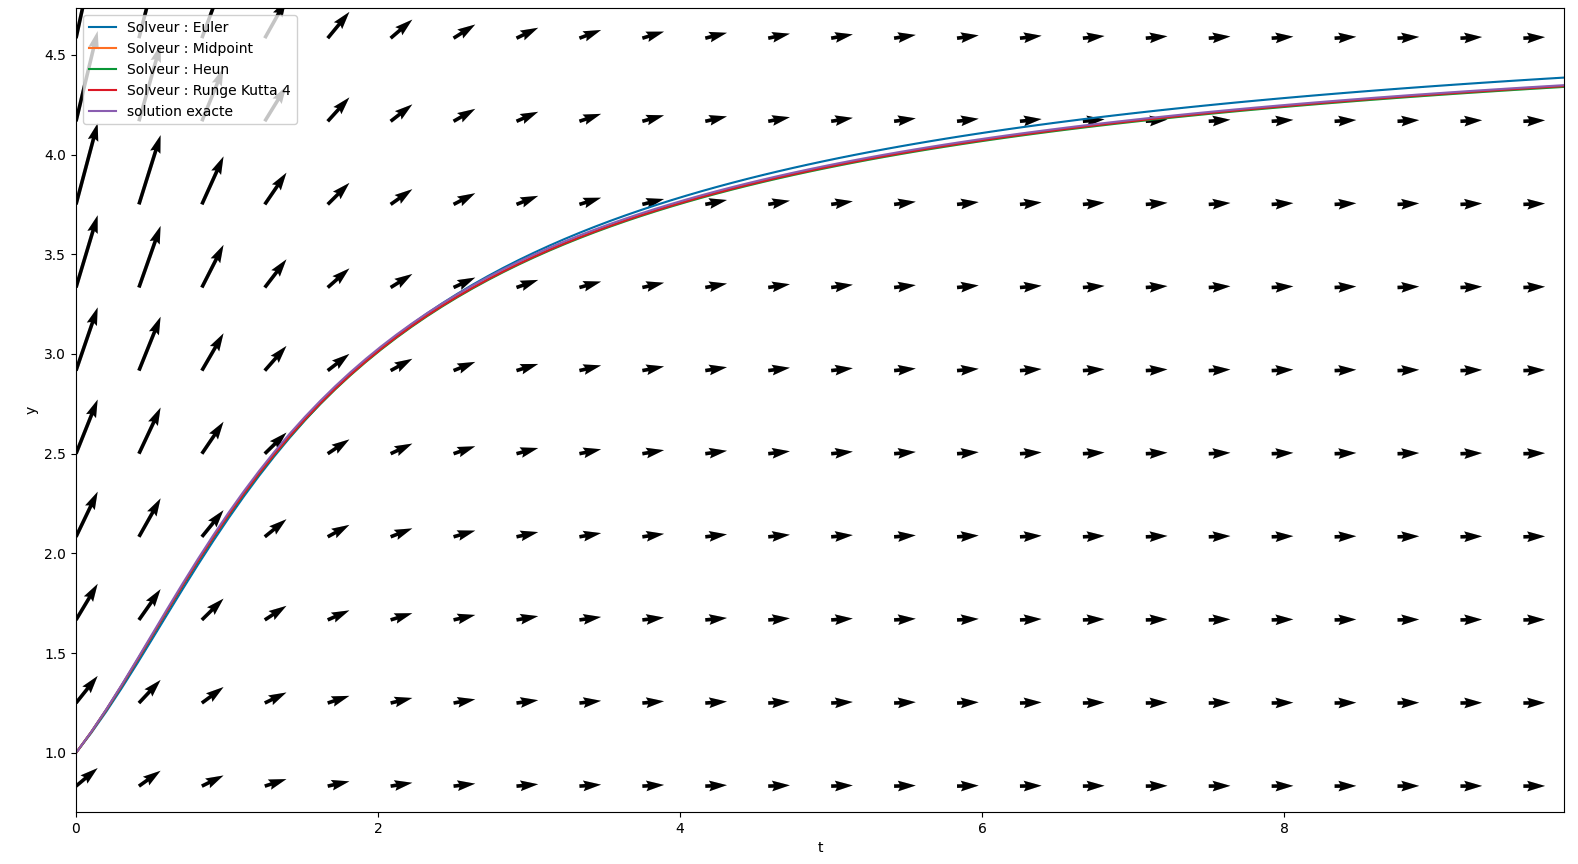
\includegraphics[width=0.49\textwidth]{img/ode1}
		\label{fig:solver_1d}
	}
	\subfloat[Résolution de $\begin{cases}
		y_1' = -y_2\\
		y_2' = y1\\
		y_1(0) = 1 \text{et} y_2(0) = 0
	\end{cases}$]{
		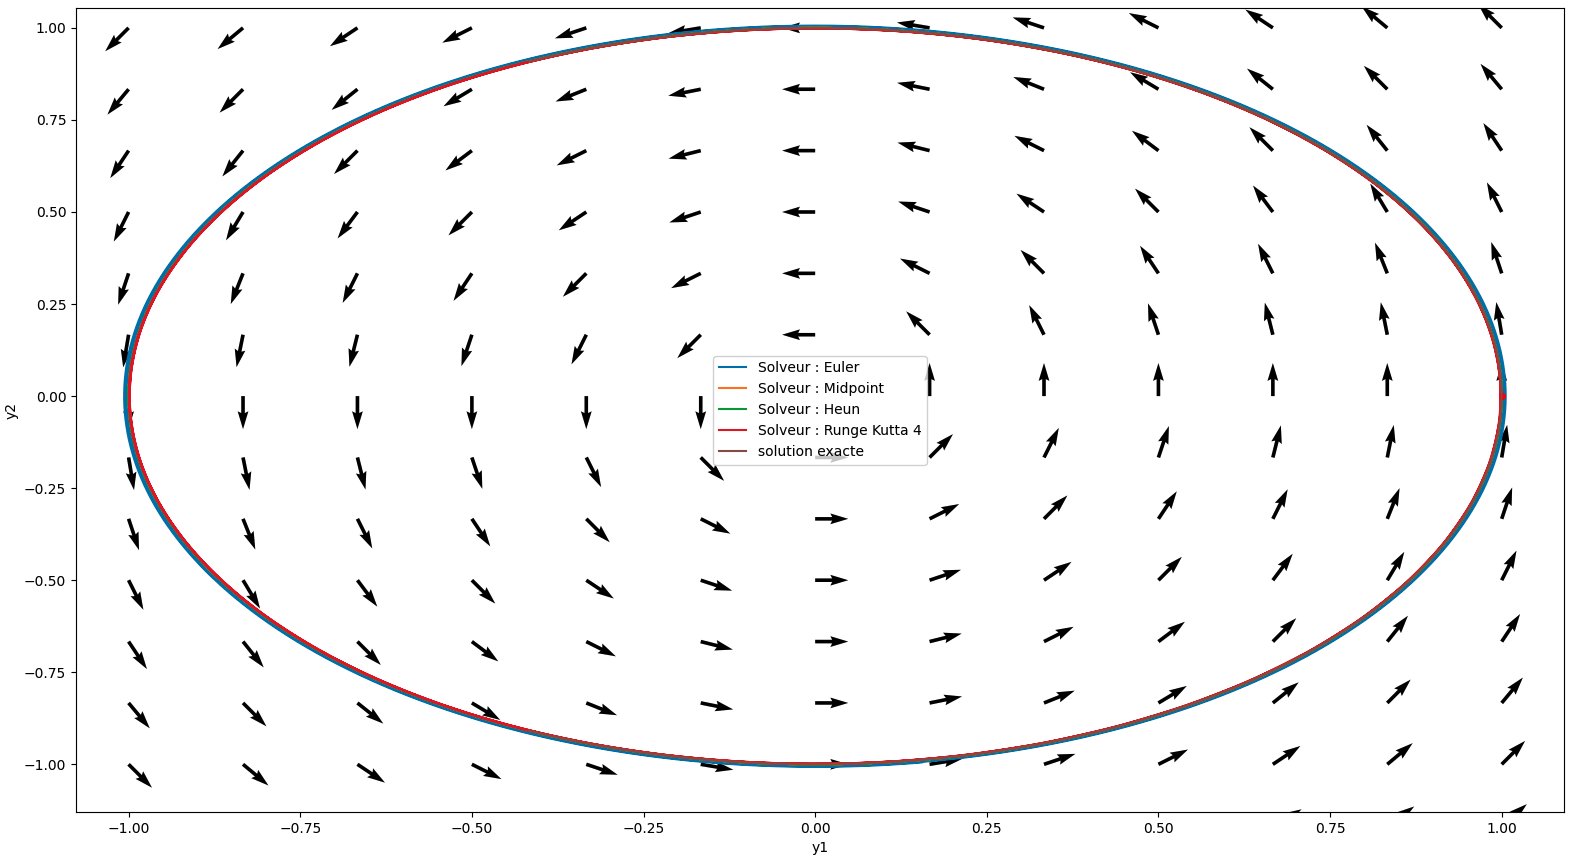
\includegraphics[width=0.49\textwidth]{img/ode2}
		\label{fig:solver_2d}
	}
	\caption{Exemples de résolution de systèmes d'équations différentielles}
	\label{fig:solver_test}
\end{figure}

On remarque en particulier que, sur la figure~\ref{fig:solver_1d}, la méthode d'Euler est bien moins performante que les autres méthodes. Cela s'explique notamment car la méthode est d'ordre 1. La méthode de Runge-Kutta étant d'ordre 4, celle-ci doit alors être préférée aux autres.\label{edo}

\section*{Système proie-prédateur de Lotka-Volterra}

Dans cette partie, nous allons nous intéresser au système proie-prédateur de Lotka-Volterra, modélisant l'évolution de la population de plusieurs espèces dans un milieu naturel.
\vskip 1mm ~

Tout d'abord, nous allons étudier les modèles de de Malthus et Verhulst. Dans ces modèles, $N(t)$ décrit la variation de la population d'un ensemble d'individus au cours du temps. $b$ représente alors le taux de naissances et $d$ le taux de décès de la population. On a alors $\gamma =b-d$ et $\kappa$ qui représente la limite des ressources. Ainsi, on peut considérer que ces modèles représentent les variations d’une population.

Nous avons pu résoudre les équations différentielles de ces modèles à l'aide la méthode de Runge-Kutta d'ordre 4.
\vskip 1mm ~

Nous nous sommes ensuite intéressés au modèle de Lotka-Volterra, constitué de deux équations différentielles. Les paramètres $a$, $b$, $c$ et $d$ représentent respectivement le taux de reproduction des proies, le taux de mortalité des proies (dû aux prédateurs rencontrés), taux de reproduction des prédateurs en fonction des proies mangées et taux de mortalité des prédateurs. Ainsi, ce modèle permet bien de modéliser un écosystème proie/prédateur.

La figure~\ref{fig:lv1} représente les variations des deux populations au cours du temps et la figure~\ref{fig:lv2} représente les variations de $(N(t), P(t))$ au cours du temps. Les solutions de ce système sont périodiques.

\begin{figure}[ht]
	\centering
	\subfloat[Variation des populations $N$ et $P$ au cours du temps]{
		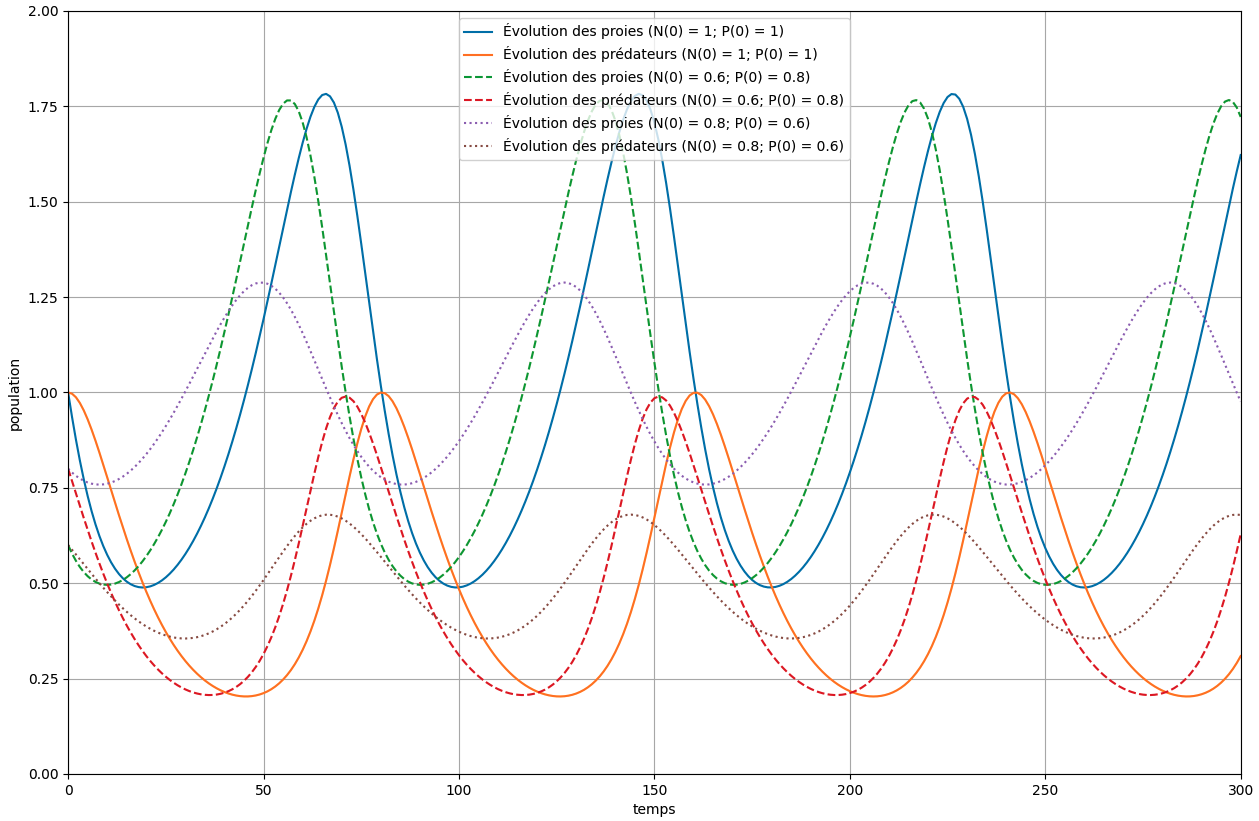
\includegraphics[width=0.55\textwidth]{img/lv1}
		\label{fig:lv1}
	}
	\subfloat[Variation de $(N(t), P(t))$ au cours du temps]{
		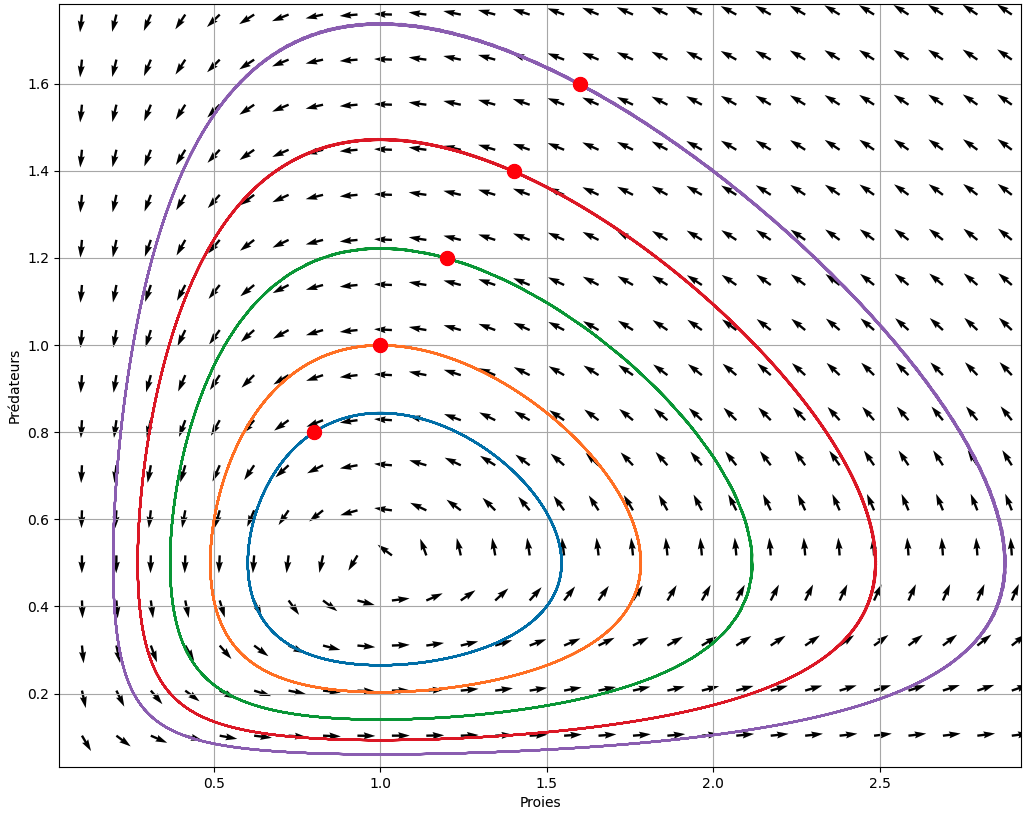
\includegraphics[width=0.44\textwidth]{img/lv2}
		\label{fig:lv2}
	}
	\caption{Résolutions du modèle de Lotka-Volterra avec différentes conditions initiales pour $a = \frac{2}{3}, b = \frac{4}{3}, c = 1 \text{ et } d =1$}
	\label{fig:lv}
\end{figure}

Les solutions étant périodiques, il est possible d'établir une estimation numérique de la période. Pour cela, nous cherchons deux maximums locaux successifs.
\vskip 1mm ~

On peut également étudier localement, sur la figure~\ref{fig:loc} les solutions autour d'un point de départ donné (ici $y_0 = [0.5,0.5]$). On remarque que les courbes des solutions ne se croisent pas.
\vskip 1mm ~

\begin{figure}[H]
	\centering
	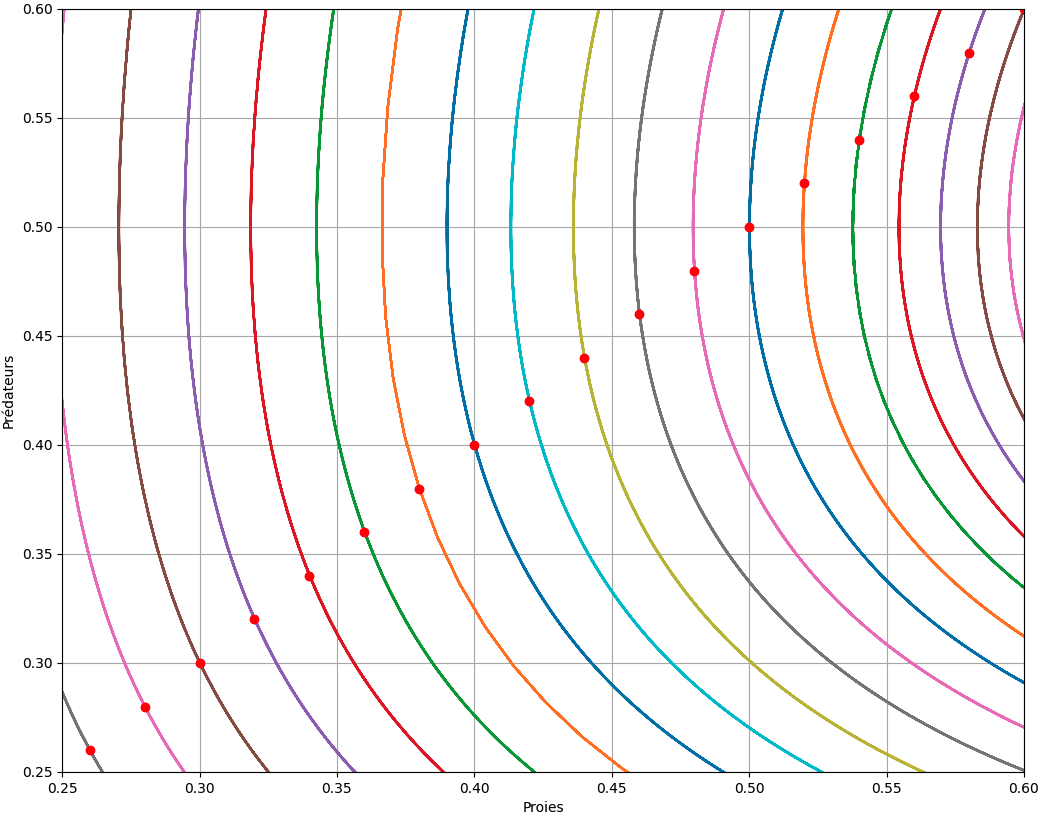
\includegraphics[width=0.5\textwidth]{img/loc}
	\caption{Étude locale de différentes solutions ayant des conditions initiales proches de $y_0 = [0.5,0.5]$}
	\label{fig:loc}
\end{figure}

Le système de Lotka-Volterra admet des points singuliers dès que les dérivées s'annulent. Ainsi, l'équation~\ref{eq:singular_points} décrit les points singuliers du système.

\begin{equation}
	\label{eq:singular_points}
	\begin{cases}
		a = bP(t)\\
		d = cN(t)
	\end{cases} \Leftrightarrow\quad
	\begin{cases}
		P(t) = \frac{a}{b} &(b \neq 0)\\
		N(t) = \frac{d}{c} &(c\neq 0)
	\end{cases}
	\quad\text{ et }\quad
	\begin{cases}
		P(t) = 0\\
		N(t) = 0
	\end{cases}
\end{equation}

Les diagrammes obtenus sont sous la forme d'orbites. Ceux-ci sont fermés. Si l'on part d'un point singulier, le système n'évolue pas. Le diagramme obtenu est alors un nuage des points singuliers.\label{lotka-volterra}

\section*{Pendule à N maillons}

Dans cette partie, nous allons nous intéresser au pendule à $N$ maillons, dont la modélisation fait intervenir des équations différentielles.
\vskip 1mm ~

Nous avons commencé par modéliser le pendule à un unique maillon. 
Pour modéliser le pendule, nous avons besoin de deux données, l'angle $\theta$ et la vitesse angulaire $\omega$.
La relation entre la dérivée de $\theta$ et $\omega$, l'expression de la dérivée de $\omega$ en fonction de $\theta$ et le problème de Cauchy sont définis dans l'équation~\ref{eq:simple_pendulum}.

\begin{equation}
	\theta' = \omega \qquad \omega' = -\frac{g}{L}\sin(\theta) \quad
	\begin{cases}
		\theta' = \omega\\
		\omega' = -\frac{g}{L}\sin(\theta)
	\end{cases}
	\label{eq:simple_pendulum}
\end{equation}

Nous avons implémenté une fonction permettant de déterminer la fréquence d'oscillation du système (\verb|determine_frequency|) en fonction de l'angle initial $\theta$. Pour cela, nous résolvons 
le problème de Cauchy défini de l'équation~\ref{eq:simple_pendulum} avec $N=10000$ et $h = \frac{10}{N}$. Après résolution, nous avons la vitesse angulaire pour $t \in [0,10]$. Ensuite,
pour calculer la période $T$, nous cherchons le premier maximum local, puis nous cherchons le second maximum local. Enfin, nous calculons la fréquence $f = \frac{1}{T}$.

La figure~\ref{fig:frequency} illustre cette fréquence pour un pendule de longueur $l=1$ et de masse $m=1$. On remarque que la fréquence est, pour de petites valeurs de $\theta$, très proche de $\frac{1}{2\pi}\sqrt{\frac{g}{l}}$. On peut donc en déduire graphiquement que, pour de petites oscillations, la fréquence est égale à $\frac{1}{2\pi}\sqrt{\frac{g}{l}}$.

\begin{figure}[ht]
	\centering
	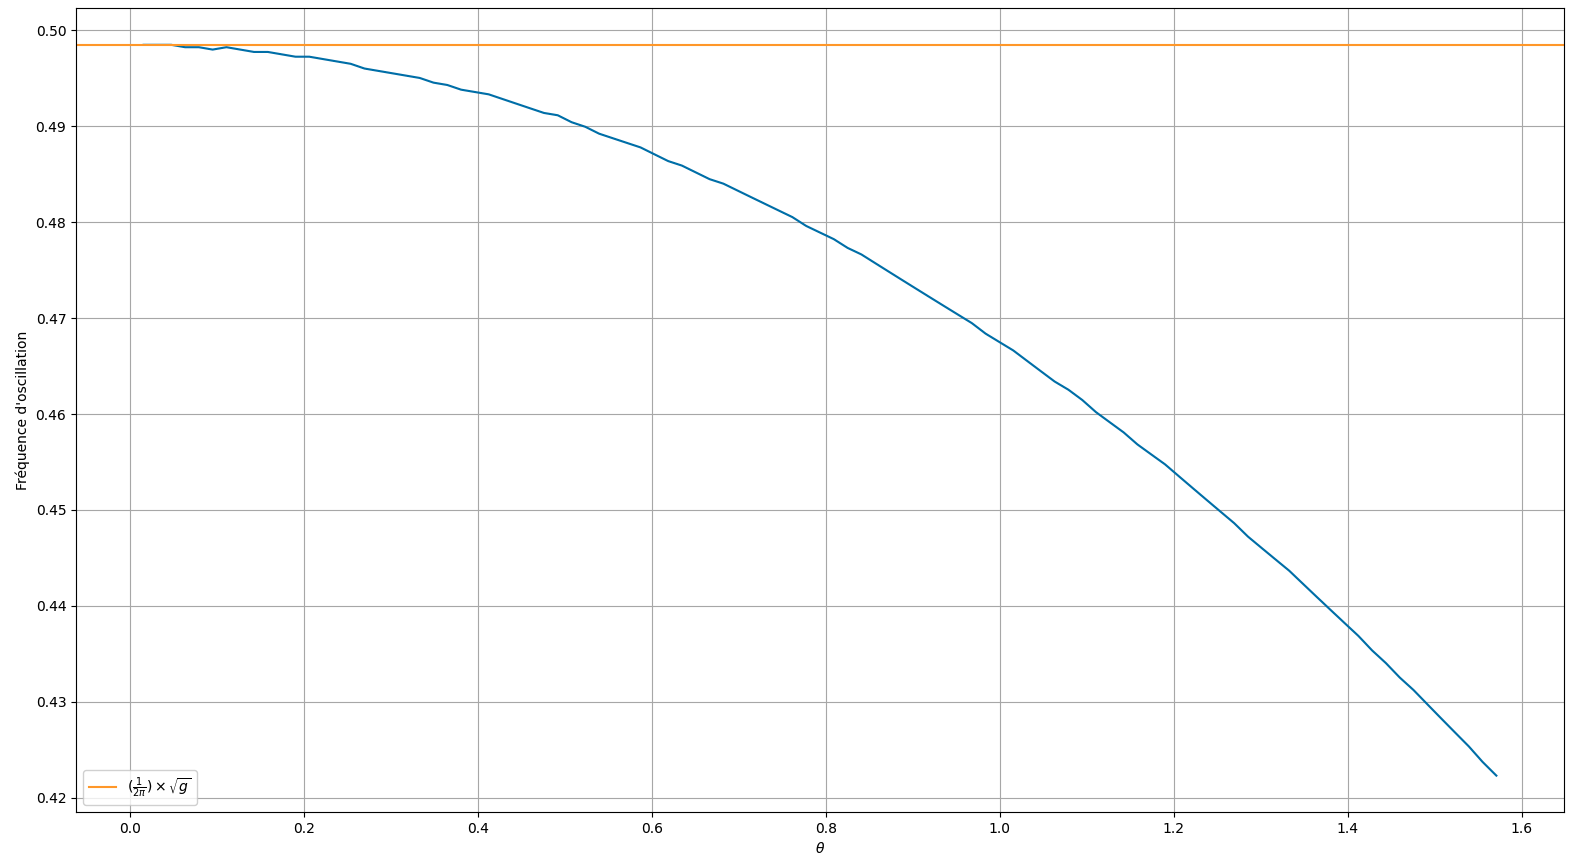
\includegraphics[width=0.6\textwidth]{img/frequency}
	\caption{Fréquence d'oscillation du pendule à un unique maillon en fonction de l'angle initial $\theta$}
	\label{fig:frequency}
\end{figure}

Ensuite, nous avons modélisé le pendule à deux maillons. Pour cela, nous nous sommes appuyés sur les équations usuelles\footnote{Source : \url{www.myphysicslab.com/dbl_pendulum.html}}.
\vskip 1mm ~

Le système à deux maillons est un système chaotique : le système dépend fortement des conditions initiales. La figure~\ref{fig:chaos}, représentant la trajectoire de l'extrémité du pendule à deux maillons en fonction du temps, illustre ce phénomène. Cette figure a été réalisée avec $50$ valeurs de $\theta$ réparties dans l'intervalle $[0,1]$. On posera alors, dans le cadre de notre modèle, $\theta_1 = \theta$ et $\theta_2 = -\theta$.

\begin{figure}[ht]
	\centering
	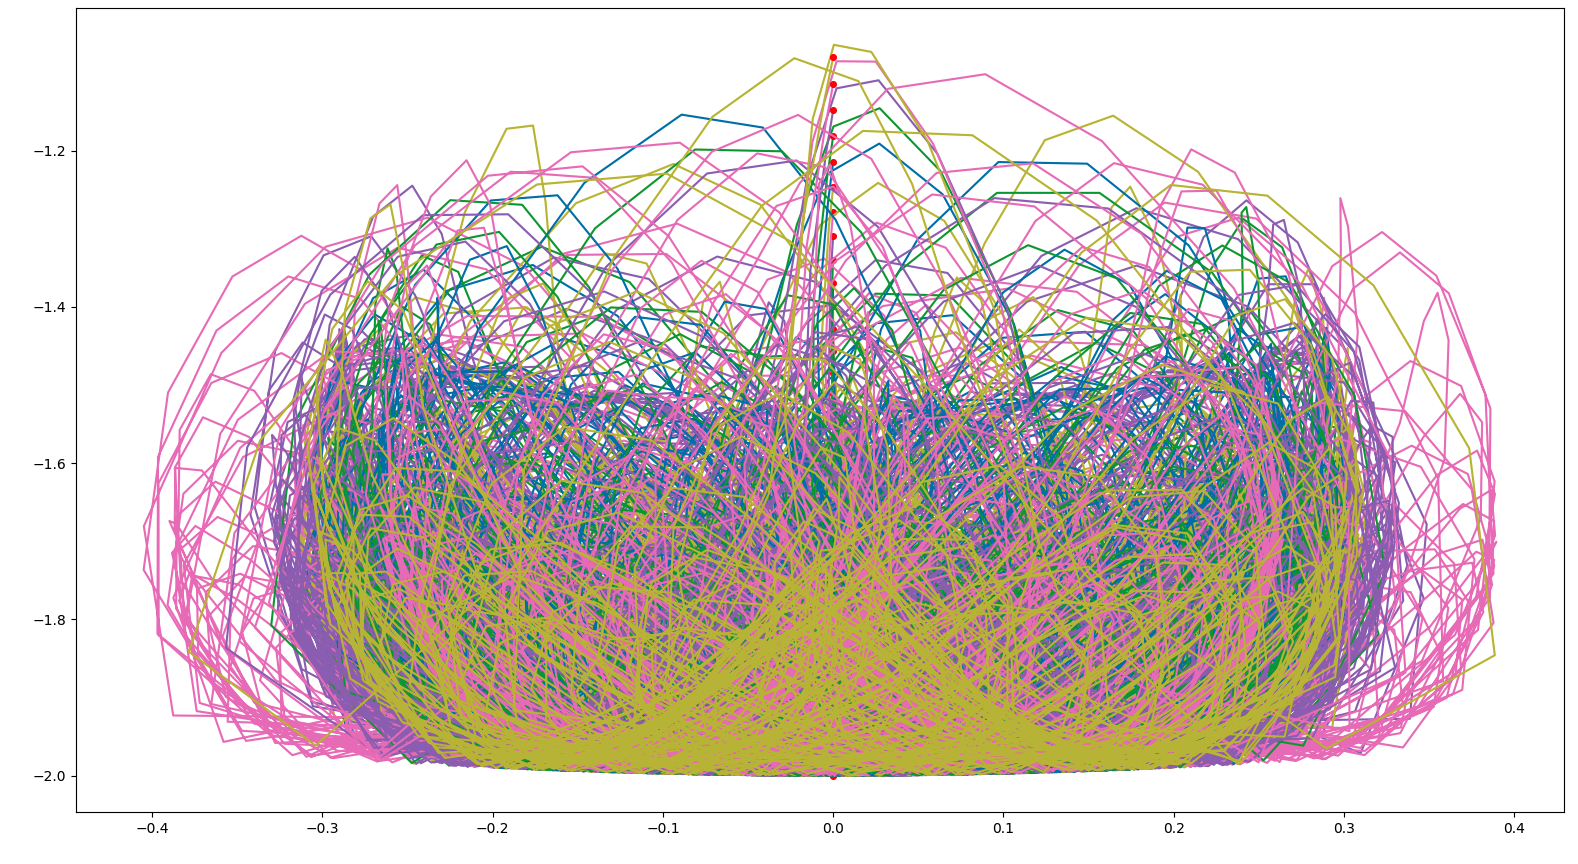
\includegraphics[width=0.6\textwidth]{img/chaos}
	\caption{Trajectoires d'un pendule à 2 maillons placé dans différentes conditions initiales}
	\label{fig:chaos}
\end{figure}

Enfin, nous avons déterminé numériquement le terme du premier retournement du pendule. Une carte représentant ce temps est représentée en figure~\ref{fig:flip_time}. Cette figure illustre bien la forte dépendance aux conditions initiales du système, chaque couleur\footnote{On retrouver la correspondances des couleurs ici : \url{https://en.wikipedia.org/wiki/Double\_pendulum\#Chaotic\_motion}} indiquant si l'un des pendules se retourne pour une période donnée.

\begin{figure}[H]
	\centering
	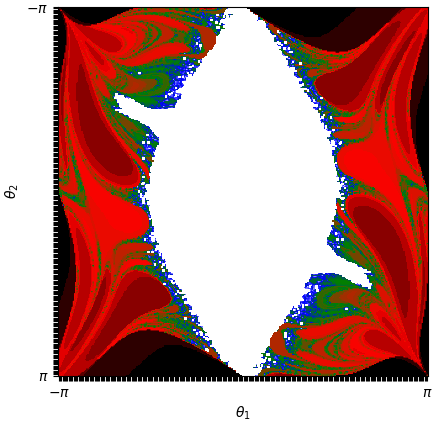
\includegraphics[width=0.60\textwidth]{img/flip_time_300x300}
	\caption{Temps de retournement du pendule en fonction des conditions initiales}
	\label{fig:flip_time}
\end{figure}\label{pendule-n-maillons}

\end{document}